\documentclass[conference]{IEEEtran}
\IEEEoverridecommandlockouts
% The preceding line is only needed to identify funding in the first footnote. If that is unneeded, please comment it out.
\usepackage{cite}
\usepackage{amsmath,amssymb,amsfonts}
\usepackage{algorithmic}
\usepackage{graphicx}
\usepackage{textcomp}
\usepackage{xcolor}
\usepackage{tikz}
\usepackage{pgfplots}
\def\BibTeX{{\rm B\kern-.05em{\sc i\kern-.025em b}\kern-.08em
    T\kern-.1667em\lower.7ex\hbox{E}\kern-.125emX}}
\begin{document}

\title{Non-compensate Recommendation Models
}

\author{Anonymous
}

\maketitle

\begin{abstract}
The study of consumer psychology reveals two categories of procedures used by consumers to make consumption related choices: compensatory rules and non-compensatory rules. Existing models assume the consumers follow the compensatory rules, which are to make decisions based on a weighted or summated score over different aspects. In this paper, we present a novel model which adopts non-compensatory decision rules. An item is selected because  (1) it is superior on the most important aspect, and (2) its performance is beyond the minimally acceptable level on other aspects. Furthermore, we incorporate other psychological concepts such as evaluation process and ordinal utility to predict consumption in activity sessions. We experimentally demonstrate that this model outperforms state-of-the-art methods.
\end{abstract}

\begin{IEEEkeywords}
conpensatory decision rules, non-compensatory decision rules, factor models 
\end{IEEEkeywords}

\section{Introduction}\label{sec:introduction}
%Recsys
\textbf{R}ecommender \textbf{S}ystem (RS) has received a lot of research attention. In the fruitful literature of RS, latent factor models are the most ubiquitous and successful  because of their superior performance. Latent factor models represent users and items as vectors of factors with the same dimensions~\cite{Gopalan2015Scalable,Hu2008Collaborative}. Inner products of the latent factor vectors of users and items are used to reconstruct the observations, which could be either point-wise values (i.e. the ratings users give to items~\cite{}) or pair-wise rankings (i.e. the order of user feedbacks~\cite{}).


%Existing work: compensate
Intuitively, a user's factors in latent factor models encode the user's ``preferences'' on some hidden ``aspects'', while an item's factors convey information about the item's ``property'' on the same aspects. The inner product describes the summated score over all aspects that a user assigns to an item. From the perspective of users, the scoring of an item is based on compensatory rules, i.e. the shortcomings of an item are balanced out by its strongpoints. For example, in the toy example 

\begin{figure}[htbp]
\begin{center}
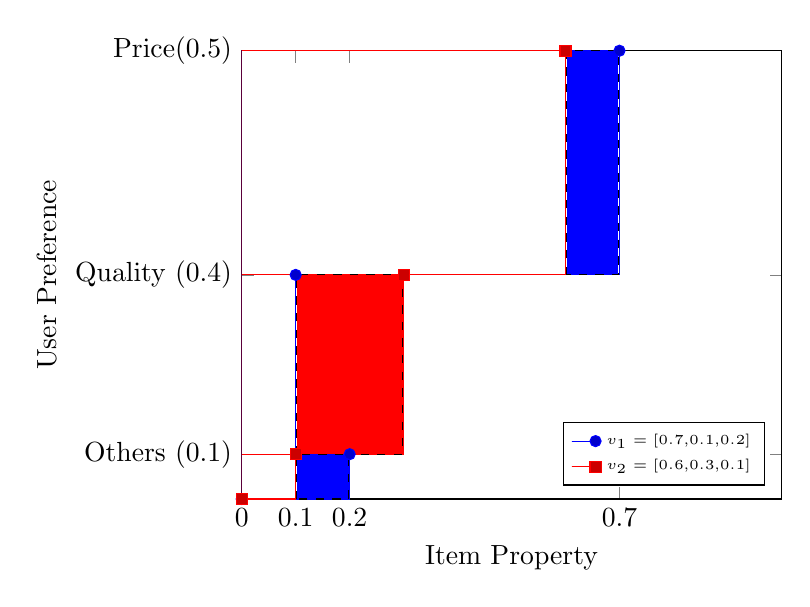
\begin{tikzpicture}
\begin{axis}[
	xmin=0,xmax=1,
%	ymin=0,ymax=1,
	ylabel=User Preference,
	every axis y label/.style={at={(ticklabel cs:0.5)},rotate=90,anchor=near ticklabel,},
	xlabel=Item Property,
	enlargelimits=false,
	ytick=data,
	xtick=data,
%	yticklabel interval boundaries,
	yticklabels={Price(0.5),Quality (0.4),Others (0.1)},
%	xbar stacked, 
%	nodes near coords,
legend style={legend pos=south east,font=\tiny},
]

\addplot+[xbar interval]
	coordinates {(0.7,1) (0.1,0.5) (0.2,0.1) (0.,0) };
\addplot+ [xbar interval] coordinates {(0.6,1) (0.3,0.5) (0.1,0.1) (0,0) };
\draw [fill=blue,dashed] (axis cs: 0.602,0.5) rectangle (axis cs: 0.698,1);
\draw [fill=red,dashed] (axis cs: 0.102,0.1) rectangle (axis cs: 0.298,0.5);
\draw [fill=blue,dashed] (axis cs: 0.102,0) rectangle (axis cs: 0.198,0.1);
\legend{$v_1=[0.7\textrm{,} 0.1\textrm{,}0.2]$,$v_2=[0.6\textrm{,}0.3\textrm{,}0.1]$}
\end{axis}

\end{tikzpicture}
\caption{Toy example: for user preference $u=[0.5,0.4,0.1]$ and items $v_1=[0.7,0.1,0.2],v_2=[0.6,0.3,0.1]$, compensatory rules prefer $v_2$ while non-compensatory rules prefer $v_1$. }
\label{default}
\end{center}
\end{figure}

Existing latent factor models in RS community are implementations of the compensatory decision rules. However, in the field of psychological science, ample evidence~\cite{Engel1986Consumer} exist to support that, despite of the compensatory rules, consumers often adopt non-compensatory rules. Non-compensatory rules do not allow a good performance on one aspect of an item to compensate for poor performances on other aspects. 



%Research problems
To the best of our knowledge, there is no RS model that is based on non-compensatory decision making rules.
In this work, we are motivated by psychological studies to build new RS models based on non-compensatory rules. We want to study the following three research questions. (1) How do we model the non-compensatory rules? (2) Do users follow the same rules for different feedbacks, i.e. explicit feedback and implicit feedback? (3) Can the model be scaled to massive recommender systems?
  
%challenge
Non-compensatory rules include lexicographic, conjunction and disjunction rules. Under lexicographic rules, products are compared on the most important aspect. Under conjunction and disjunction rules, the consumer imposes requirements for minimally acceptable values on each aspect separately. The conjunction and disjunction rules are often used in conjunction with lexicographic rules.
  
%For explicit feedback
Explicit feedback. graded implicit feedback.  

%For implicit feedback
Binary implicit feedback. 

%Algorithm
For the above two models, we propose 

%Contribution
Our contributions are three folds. (1) for explicit and graded sessional feedback. (2) for binary implicit feedback. (3) highly parrallel inference algorithm. 

%Paper structure
This paper is structured as follows. We briefly introduce related work in Sec.~\ref{sec:relatedwork}. The main contributions of this paper are described in Sec.~\ref{sec:model1} to Sec.~\ref{sec:algorithm}. The complete non-compensate model for explicit and graded sessional feedback is presented in Sec.~ref{sec:model1}. The simplified non-compensate model for binary implicit feedback is presented in Sec.~\ref{sec:model2}. The highly parrallel algorithm is presented in Sec.~\ref{sec:algorithm}. We analyze experimental results on real recommendation data sets in Sec.~\ref{sec:experiment}. Finally, we conclude our work and give future directions in Sec.~\ref{sec:conclusion}. 


\section{Related Work}\label{sec:relatedwork}
%factor models

%rating v.s. ranking based

%implicit feedback

\section{Complete Non-compensate Rules for Explicit Feedback}\label{sec:model1}

\section{Simplified Non-compensate Rules for Implicit Feedback}\label{sec:model2}

\section{Highly Parrallel Inference}\label{sec:algorithm}

\section{Experiment}\label{sec:experiment}

\subsection{Experimental Setup}

\subsection{Comparative Performance on Explicit Feedback}

\subsection{Comparative Performance on }


\section{Conclusion}\label{sec:conclusion}
\section*{References}

Please number citations consecutively within brackets \cite{b1}. The 
sentence punctuation follows the bracket \cite{b2}. Refer simply to the reference 
number, as in \cite{b3}---do not use ``Ref. \cite{b3}'' or ``reference \cite{b3}'' except at 
the beginning of a sentence: ``Reference \cite{b3} was the first $\ldots$''

Number footnotes separately in superscripts. Place the actual footnote at 
the bottom of the column in which it was cited. Do not put footnotes in the 
abstract or reference list. Use letters for table footnotes.

Unless there are six authors or more give all authors' names; do not use 
``et al.''. Papers that have not been published, even if they have been 
submitted for publication, should be cited as ``unpublished'' \cite{b4}. Papers 
that have been accepted for publication should be cited as ``in press'' \cite{b5}. 
Capitalize only the first word in a paper title, except for proper nouns and 
element symbols.

For papers published in translation journals, please give the English 
citation first, followed by the original foreign-language citation \cite{b6}.

\begin{thebibliography}{00}
\bibitem{b1} G. Eason, B. Noble, and I. N. Sneddon, ``On certain integrals of Lipschitz-Hankel type involving products of Bessel functions,'' Phil. Trans. Roy. Soc. London, vol. A247, pp. 529--551, April 1955.
\bibitem{b2} J. Clerk Maxwell, A Treatise on Electricity and Magnetism, 3rd ed., vol. 2. Oxford: Clarendon, 1892, pp.68--73.
\bibitem{b3} I. S. Jacobs and C. P. Bean, ``Fine particles, thin films and exchange anisotropy,'' in Magnetism, vol. III, G. T. Rado and H. Suhl, Eds. New York: Academic, 1963, pp. 271--350.
\bibitem{b4} K. Elissa, ``Title of paper if known,'' unpublished.
\bibitem{b5} R. Nicole, ``Title of paper with only first word capitalized,'' J. Name Stand. Abbrev., in press.
\bibitem{b6} Y. Yorozu, M. Hirano, K. Oka, and Y. Tagawa, ``Electron spectroscopy studies on magneto-optical media and plastic substrate interface,'' IEEE Transl. J. Magn. Japan, vol. 2, pp. 740--741, August 1987 [Digests 9th Annual Conf. Magnetics Japan, p. 301, 1982].
\bibitem{b7} M. Young, The Technical Writer's Handbook. Mill Valley, CA: University Science, 1989.
\end{thebibliography}
\vspace{12pt}
\color{red}
IEEE conference templates contain guidance text for composing and formatting conference papers. Please ensure that all template text is removed from your conference paper prior to submission to the conference. Failure to remove the template text from your paper may result in your paper not being published.

\end{document}
